\documentclass[../main.tex]{subfiles}
\graphicspath{{\subfix{../images/}}}

\begin{document}

\begin{newrequirements}
    \begin{todolist}
    \item[\done] Actual Design description with pictures 
        and diagrams. E.g., a “wiring diagram” 
        of the implemented hardware can be 
        added. 

	\item[\done] Actual images of various modules must 
        be included wherever possible. 
        Otherwise, at least the images of 
        various aspects of the completed design 
        must be shown. 

    \item[\done] List the different tools and framework 
        used for the implementation. 

    \item[\done] Discuss any novel aspects of your 
        implementation (if applicable). You may 
        link this aspect of your design to the 
        comparison table at the end of 
        literature review and elaborate on the 
        steps taken in achieving these 
        novelties in your design. 

    \item[\done] Discuss the challenges encountered 
        during the implementation and how they 
        were addressed. 

    \item[\done] You may organize any of the above 
        recommended points as subsections 

    \end{todolist}
\end{newrequirements}
In this section are going illustrate the actual design 
implementations, to achieve the design solution.
\subsection{Hardware}

The most critical parts in the hardware
architecture are the Raspberry Pi and the drone. 
We started by configuring the Raspberry Pi micro\textsc{sd} card,
flashed it with Ubuntu 20.04 desktop version,
and installed Parrot Olympe successfully in virtual environment. 
Then, we plugged in the Wi-Fi dongle adapter
in a \textsc{usb}~2.0 port in the Raspberry Pi, 
and the \textsc{os} discovered it automatically. 
There were some challenges in setting up the connection automatically 
once the Raspberry Pi boots up. We discovered that some packages were not installed properly,
so we reinstalled the whole system again, and the problems has been addressed. 


Regarding the power supply, we were thinking 
of modifying the drone's battery by removing the 
plastic shield because of the drone's payload restrictions 
and limitations, but everything changed after testing 
the drone's maximum payload.
As far as the connection, there are 
two different options as shown in \cref{fig:connection}.
For option A we can use \textsc{usb}-A to power the Raspberry directly 
without needing to solder any wires, but there is some internal resistance.
In option B, it powers the Raspberry Pi through the \textsc{gpio} 
interface by soldering two wires to the power board and 
connecting to pin 4 and 6 in the Raspberry Pi board.
This option has smaller internal resistance compared to option A.
For simplicity, we chose option A and   
followed the instruction of the manufacturer by choosing 
the thickest and shortest possible \textsc{usb} cable to reduce 
the power loss and voltage drops~\cite{makerfocus}.

As shown in \cref{fig:connection} We have printed the 3d 
parts, and because we need lightweight and strong parts, 
we have used PETG material with a 45\% fill rate, 
then we used superglue to stick all the parts together 
and make sure it's one solid piece.

\begin{figure}[p]
	\centering
	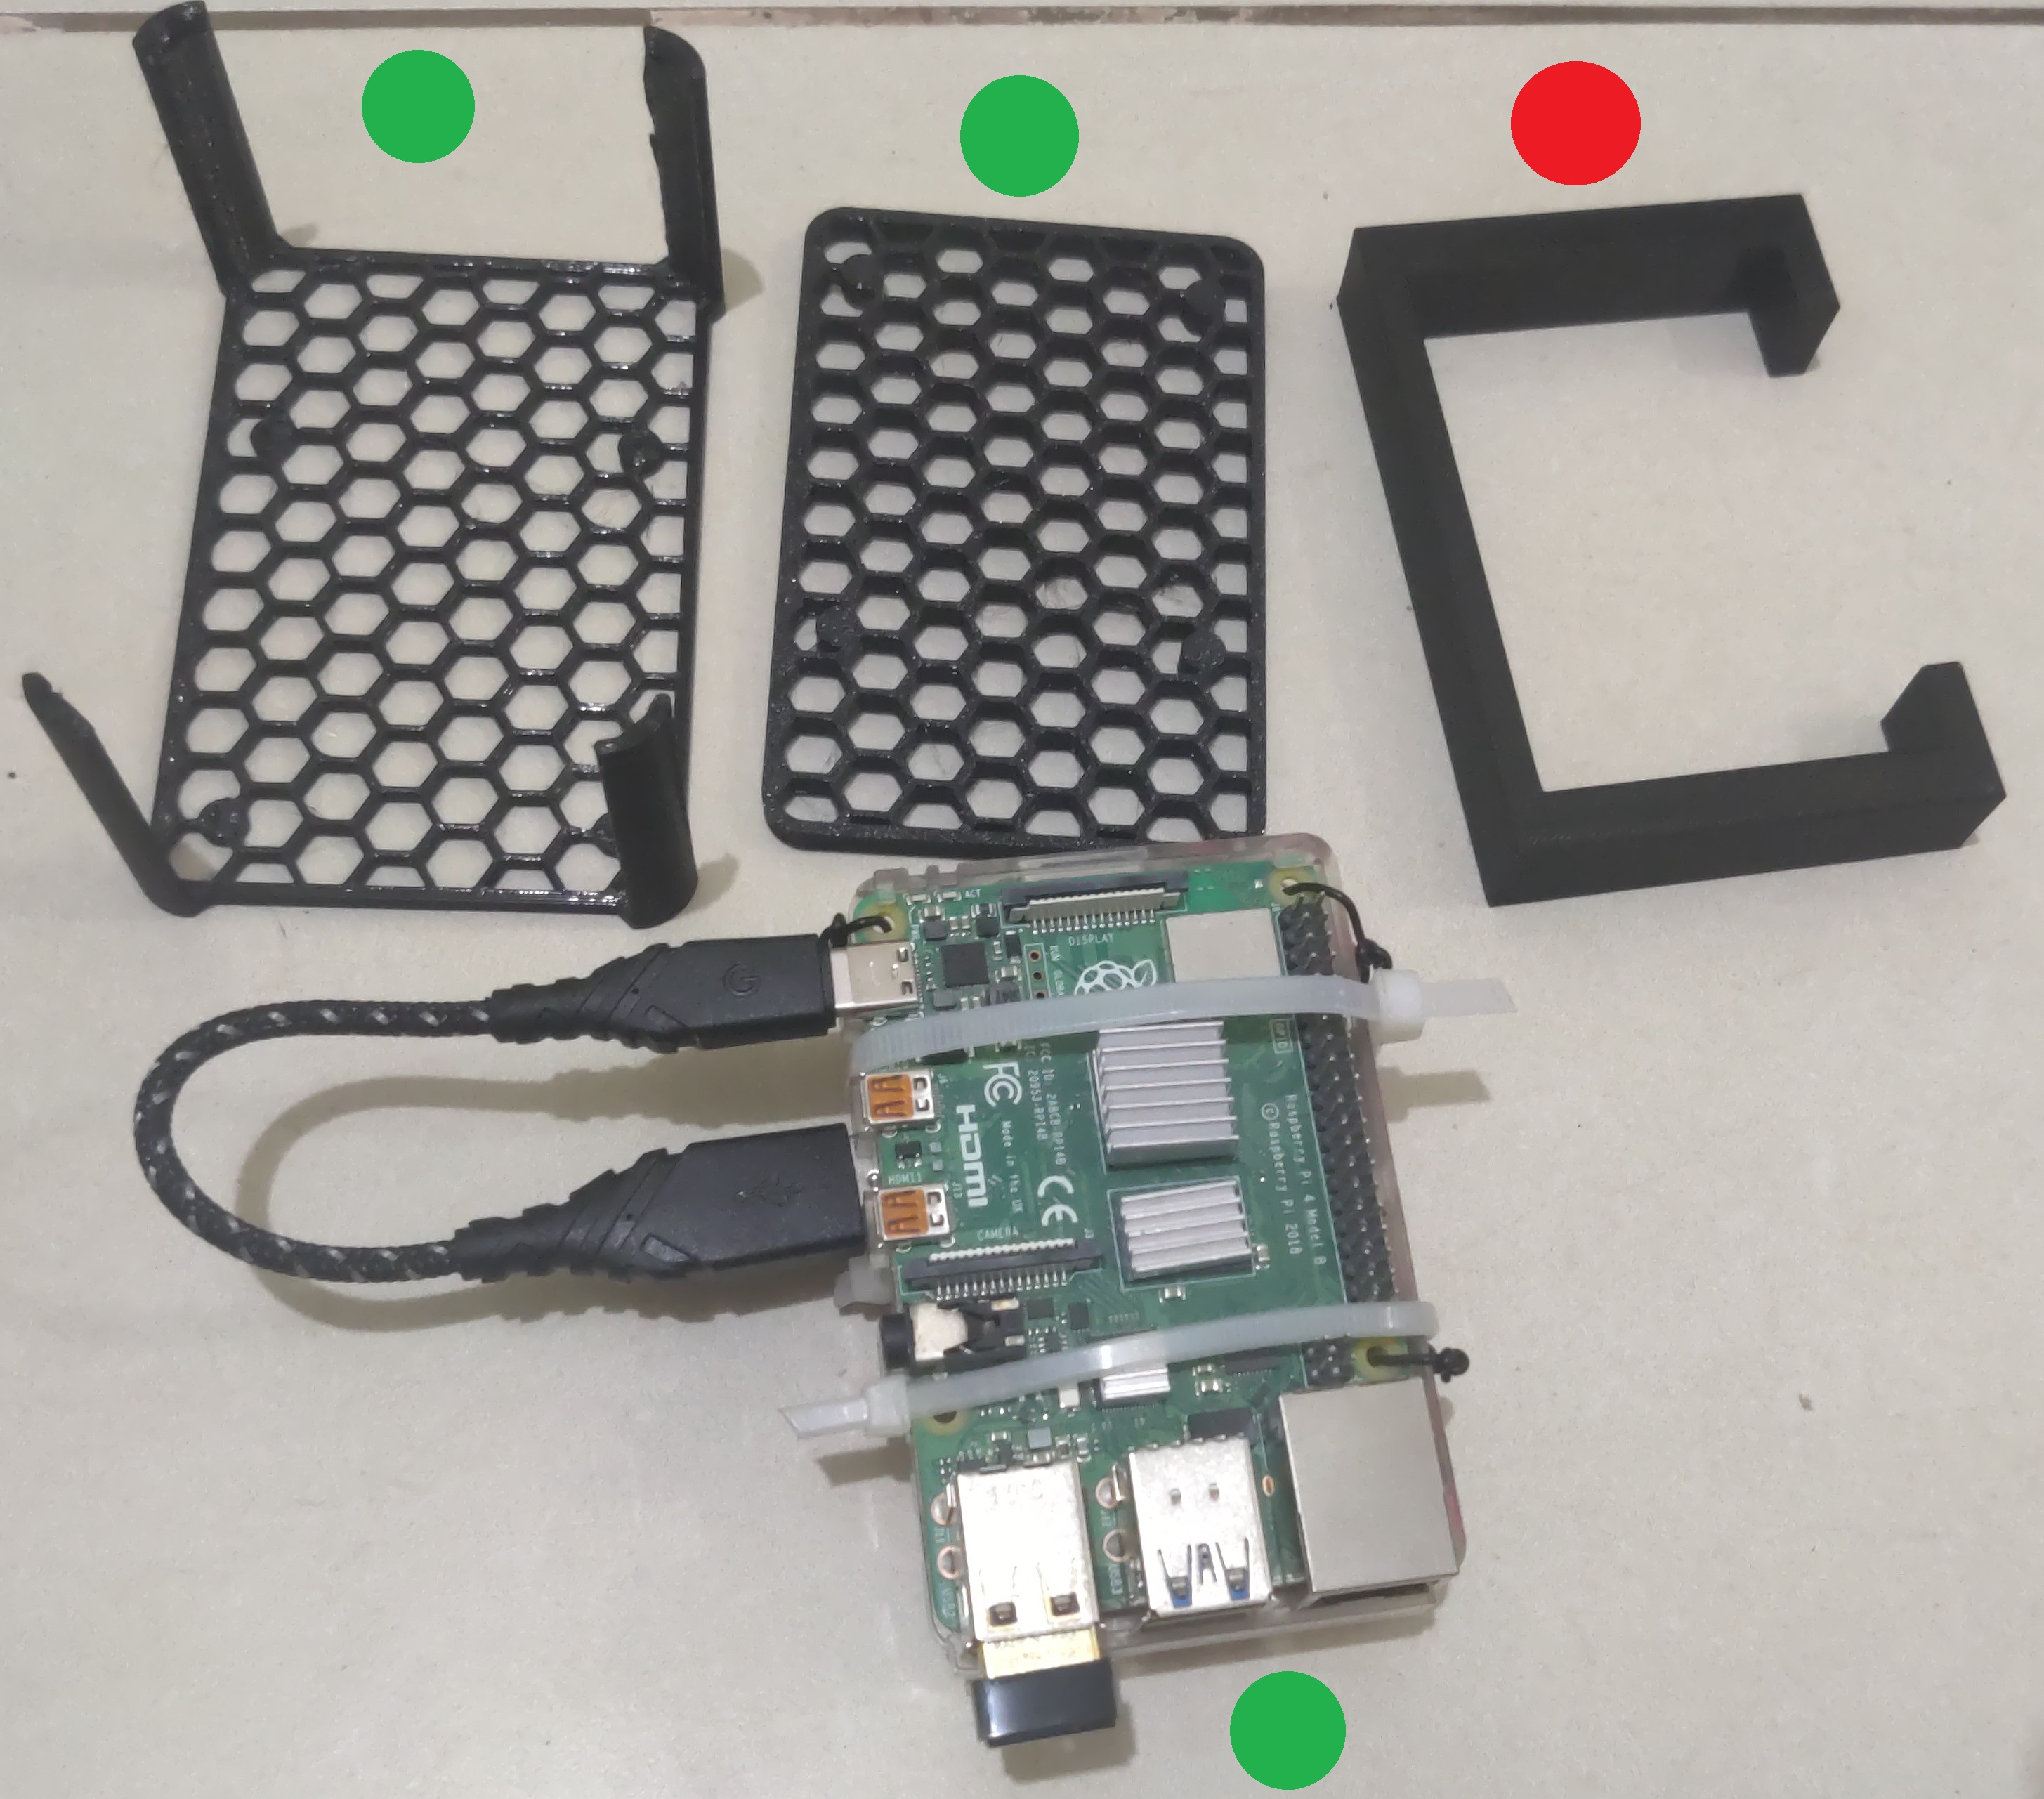
\includegraphics[width=0.5\textwidth]{parts.jpg}
	\caption{3d printed parts \& on-board computer}
	\label{fig:printed-parts}
\end{figure} 

\begin{figure}[p]
	\centering
	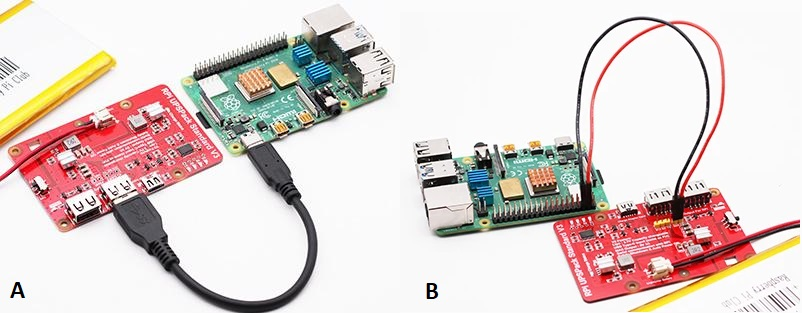
\includegraphics[width=0.5\textwidth]{connection.png}
	\caption{The Raspberry Pi and power board connection.}
	\label{fig:connection}
\end{figure}  

Since all the components are available as shown 
in \cref{fig:components}, we could assemble 
all the parts in one piece and started testing the whole system.
We have used the zip tie to hold the components and to
make sure everything sticks together. Then we put them in the 3d
printed case. As shown in 
\cref{fig:full-hardware}, all the parts are in one system. 
While testing it, the drone struggled to take off and balance itself
because the total weight exceeded the limit. So we
only used the on that are marked with a green dot 
as shown in \cref{fig:components} and the weight reduced to \SI{193}{gram}. 
Now the drone takeoff is normal, but the drone faces difficulty moving normally ,so we removed all 3D parts, and now the drone moves normally.


\begin{figure}[p]
	\centering
	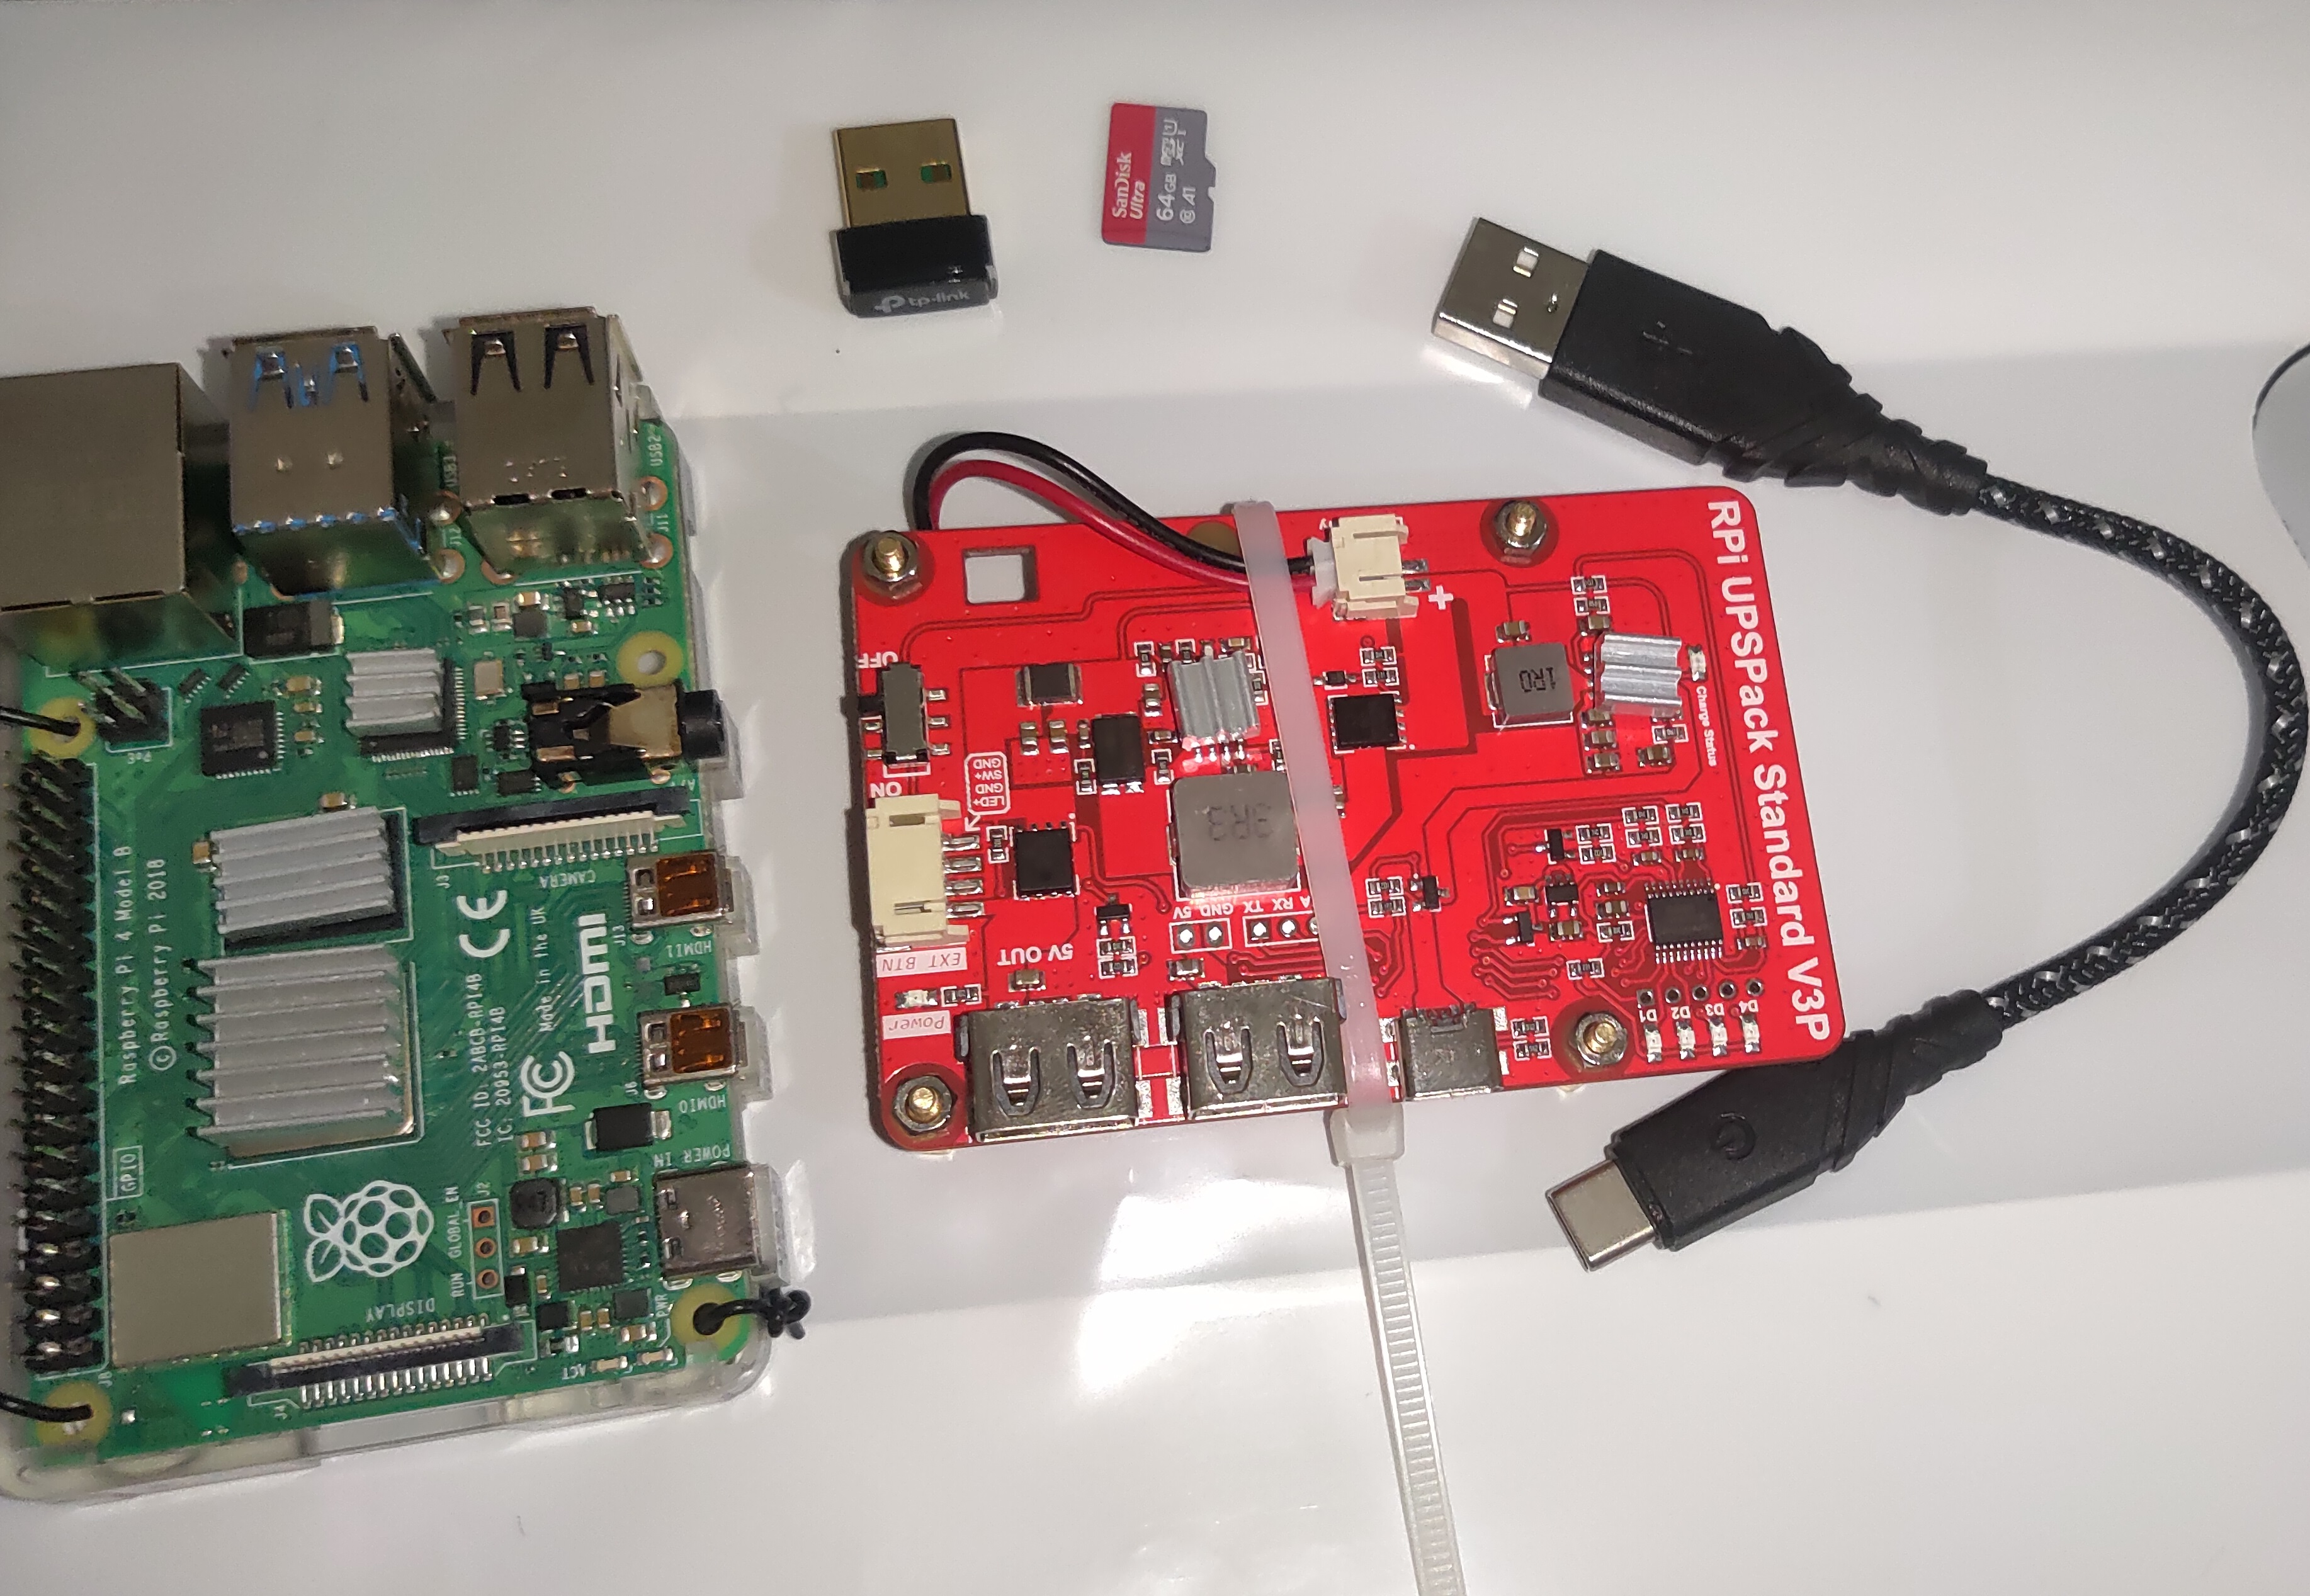
\includegraphics[width=0.5\textwidth]{components.jpg}
	\caption{All components needed.}
	\label{fig:components}
\end{figure}

\begin{figure}[h]
	\centering
	\includegraphics[width=0.7\textwidth]{fulldronehardware.png}
	\caption{Full hardware system.}
	\label{fig:full-hardware}
\end{figure}  



\subsection{Reinforcement learning}

\subsubsection{Algorithm}

We have used the state-of-the-art \gls{ppo} algorithm as our \gls{rl}
model. 
It shares features with many other actor-critic algorithms such
as the \gls{a2c} on which \gls{ppo} directly improves~\cite{ppo}.
The main reason we have chosen it over the others is that it restricts
the objective function's updates just like \gls{trpo}, but it does so
in a simpler and more effective way through clipping~\cite{ppo}.
This is an important consideration because updates in \gls{rl} are
notoriously unstable~\cite{Hen18}. 

While \cref{tab:ppo-features} lists the original features of \gls{ppo},
many frameworks have added their own improvements on the algorithm.
We are using the \gls{ppo} implementation by Stable~Baselines~3
which adds advantage normalization and value function clipping%
~\cite{sb3}.
Both of these additional features contribute further to the stability
of the training.

\begin{table}[H]
    \centering
    \caption{The main features of \gls{ppo} and their brief
    descriptions~\cite{ppo}.}
    \label{tab:ppo-features}
    \begin{tabularx}{\textwidth}{ X p{12.3cm} }
        \toprule
            \textit{Feature} 
                & \textit{Description}\\

        \midrule
        Actor-critic
                & 
                Learns both a policy and a value function which
                complement each other. 
                While the policy network (actor) chooses an action
                stochastically, the value function network (critic)
                judges how good the action is and adjusts the policy
                network updates accordingly. 
                \\ \addlinespace
        
        TD lambda
                & 
                Balances the variance and bias very well by allocating
                weights to all actions in a trajectory according to
                the hyperparameter $\lambda$ in estimating the
                state-value function. 
                \\ \addlinespace

        \gls{gae}
                & 
                Uses the TD lambda to estimate the advantage function
                which is used as the target and baseline in \gls{ppo}.
                This further reduces the variance of the target in
                exchange for some bias.
                \\ \addlinespace
        
        Buffer
                & 
                Allows the agent to collect experiences and save them
                in the buffer.
                The agent then trains the networks on the mini-batches
                sampled from this buffer.
                Consequently, it makes mini-batches more \gls{iid}.
                \\ \addlinespace

        Workers
                & 
                Allows the agent to explore different environments at
                the same time through multiple synchronous vectorized
                workers.
                It is imperative to make the seeds of these
                environments different so that they act differently
                from each other making the agent really exploit the
                multiple workers
                \\ \addlinespace
        
        Clipping
                & 
                Restricts the objective function updates.
                If the update is higher than 1-$\epsilon$ and the
                action is good, the update variable $r$ should be set
                to 1-$\epsilon$ and not more.
                Otherwise, if the action is bad and the update is
                higher than 1-$\epsilon$, also limit the update
                variable $r$ to 1-$\epsilon$.
                \\ \addlinespace
        
        \bottomrule
    \end{tabularx}
\end{table}

\Cref{tab:hyperparameters} shows the hyperparameters we have used in
the training for the fixed-targets and mobile-targets missions
respectively.
Hyperparameters in \gls{rl} matter more than in \gls{sl}, so we have
paid an extra attention to setting the correct
values~\cite{hyperparameters}.
This is another reason we have chosen the stable \gls{ppo}
algorithm and the specific implementation described above.
This means that hyperparameters have less influence in our training
compared to if we had used algorithms that are not stable such as 
\gls{dqn} and its variants.

Since there is no tried and true methods to decide on the values of
the hyperparameters,  we have consulted similar missions such as the frozen
lake and lunar lander and observe what have worked after thousands of
trials by the community.
The reason the fixed-targets and mobile-targets have different
hyperparameters is due to the fact that
most hyperparameters are a trade off between faster learning and a
stable learning.
For example, making the learning rate high will cause the agent to
learn faster but it will lose prior knowledge from previous
observation, and thus learning becomes unstable.
Similarly, a low buffer size saves time but is less stable. 
Therefore, considering the mobile targets are more complex than the
static targets, the hyperparameters are different to make its training
more stable.

\begin{table}[H]
    \centering
    \caption{Hyperparameters used during the training.}
    \label{tab:hyperparameters}
    \begin{tabularx}{0.8\textwidth}{ X l l }
        \toprule
        \textit{Hyperparameter} 
            & \textit{Fixed-targets mission} 
                & \textit{Mobile-targets mission} \\

        \midrule
        
        Total timesteps
            & 50,000 
                & 100,000 
                \\
        Buffer size 
            & 1024 
                & 2048 
                \\
        
                \raggedright Max timestep per \newline 
                \hphantom{M} episode
            & 15
                & 20
                \\

        Learning rate
            & 0.003
                & 0.0003
                \\
        
        Reward scale
            & 1.5 
                & 1.5 
                \\

        Batch size
            & 64
                & 64
                \\

        \bottomrule		
    \end{tabularx}
\end{table}

\subsubsection{Targets' movements}

\paragraph{Fixed-targets mission}

The initial positions of the targets are generated from a skewed
multivariate normal distribution using the Scipy library in Python
shown in Fig.~\ref{fig:position-distribution}.
After every episode, new positions are generated.

\begin{figure}[!t]
	\centering
	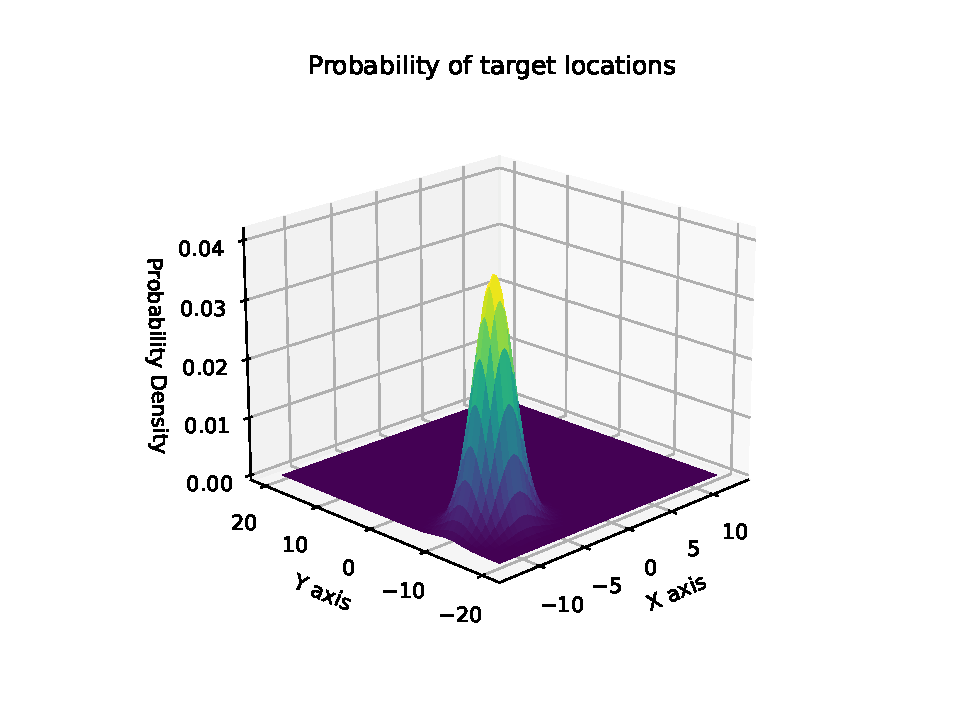
\includegraphics[width=0.8\textwidth]{target-distribution}
	\caption{The distribution of the initial positions of the
            targets in the fixed targets mission. The x-y plane
            corresponds to the ground, and the drone faces the positive
            x-direction throughout the mission.}
	\label{fig:position-distribution}
\end{figure}

\paragraph{Mobile-targets mission}

When it comes to the mobile targets mission, we have set only three of
the 10 targets to be mobile and the rest fixed for several reasons.
Firstly, we would like to be able to perform the integration testing
replicating the visual simulation, and so three of us can control or
monitor the three mobile targets accurately and effectively.
Secondly, we would like to see how the agent will react with having a
mixed of fixed and mobile targets.
Finally, we anticipated that the higher the number of mobile targets, the 
longer the training time. 
Therefore, training for a mission where all of the targets are mobile
might not be feasible given our weak computer and the \textsc{sdp}
timespan.

Similar to the fixed-targets mission,
new positions are generated after every episode.
The initial positions of the fixed targets are generated from 
the distribution shown in
\cref{fig:fixed-position-distribution}
while mobile targets from the distribution shown in
\cref{fig:mobile-position-distribution}.

\begin{figure}[!t]
	\centering
        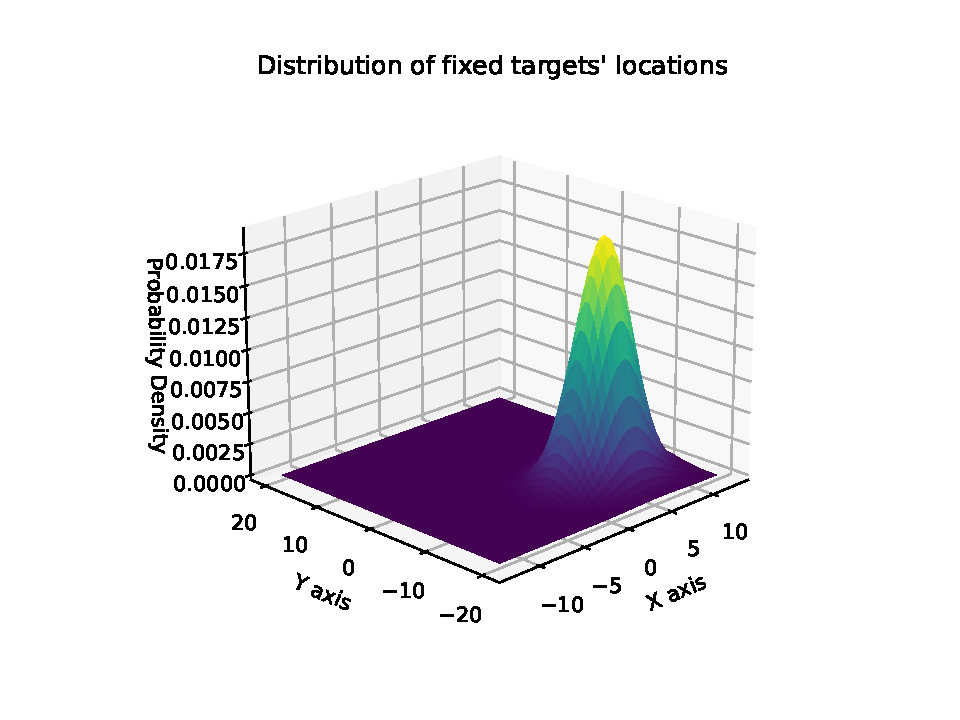
\includegraphics[width=0.8\textwidth]{fixed-target-distribution}
	\caption{The distribution of the initial positions of the
        fixed targets in the mobile-targets mission.}
	\label{fig:fixed-position-distribution}
\end{figure}

\begin{figure}[!t]
	\centering
	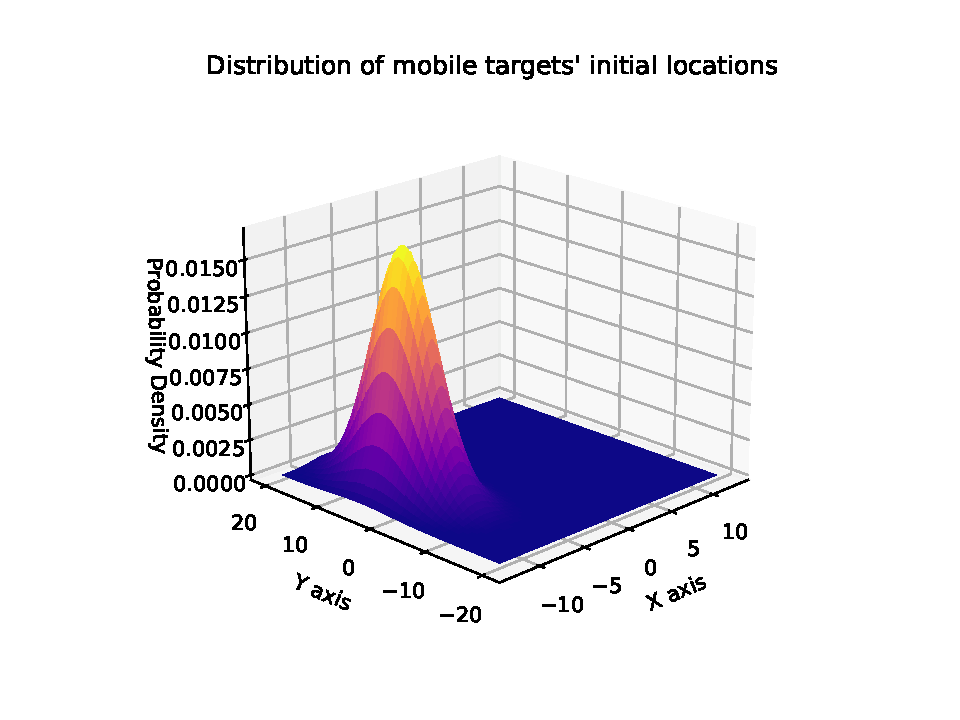
\includegraphics[width=0.8\textwidth]{mobile-target-distribution}
	\caption{The distribution of the initial positions of the
            mobile targets in the mobile-targets mission.}
	\label{fig:mobile-position-distribution}
\end{figure}

In addition, their movements consist of eight discrete
actions: forward, backward, left, right,
forward-left, forward-right, backward-left and backward-right.
A new movement is chosen after the previous one has lasted for 1 meter
or the target has reached a boundary.
We have made the targets such that they choose to move 70\% 
of the time forward-left (north-west) and 30\% of the time divided
among the remaining seven directions.

\subsubsection{Challenges}

In \cref{tab:rl-challenges}, we list the challenges we have
encountered while developing the simulation and \gls{rl} and the ways
we have tried to address them.

\begin{center}
    \begin{xltabular}{\textwidth}{ X X }
        \caption{Challenges and our attempted solutions in simulation and
        \textsc{rl} parts of the project.} 
        \label{tab:rl-challenges} \\

        \toprule
        \textit{Challenge} 
            & \textit{Solution} \\

        \midrule
        \endfirsthead
        \caption[]{Challenges and our attempted solutions in simulation and
        \textsc{rl} parts of the project (continued)} \\

        \toprule
        \textit{Challenge} 
            & \textit{Solution} \\

        \midrule
        \endhead
        
        In coding the behaviour of the targets, there were many
        incompatibilities in the versions of the C/C++ libraries that
        Sphinx requires and those available on Ubuntu 18.04.
            & 
        If the incompatibilities are trivial, we simply symlinked the
        required library to what is available on Ubuntu 
        (e.g.~\texttt{libboost}).
        Otherwise, we used Docker to create the right \textsc{os} 
        environment and worked in the container 
        (e.g.~\texttt{libgazebo}). 
            \\ \addlinespace

        Sphinx has a known bug of memory leak that is caused by the
        simulated camera storage and by not recognizing the presence
        of some \textsc{gpu}s and their drivers.
        This problem led to Sphinx occupying the entire \textsc{ram} and 
        Swap space thus crashing the system after about 10 minutes.
        So, training was impossible unless this was solved.
            & 
        Our solution for the camera storage during the training was to
        replace the camera with another communication channel between the
        targets and the agent.
        If the agent arrives at a cell, the targets in that cell will
        inform the agent of their presence.
        For the \textsc{gpu} and its driver, we have managed to set up
        one of our laptops in such a way that played nicely with
        Sphinx, so we used it for the training.
            \\ \addlinespace

        The training required a powerful computer and took a long
        time.
            & 
        The laptops that we had were too weak for the training task. 
        At first, we resorted to using the QU's research server which
        has powerful \textsc{cpu} and \textsc{gpu} but the \textsc{its}
        frequently reset our access, so this method was unreliable.
        We also tried using a remote \textsc{gpu}-optimized
        \textsc{vm} which was charged based on pay-as-you-use.
        However, the memory leak problem as described above kept
        occurring on the \textsc{vm}.
        The only solution left for us was to use our personal laptop
        to train the agent, but we had to organize our time well to
        avoid being late.
            \\ \addlinespace

        One of the unique features of the \gls{ppo} algorithm is the
        ability of the agent to mobilise multiple workers to collect
        experiences. 
        However, Sphinx would not allow multiple drones to be spawned
        in different environments at the same time.
            & 
        There was nothing we could do about this so we resorted to
        using \gls{ppo} without this feature.
            \\ \addlinespace

        \bottomrule		
    \end{xltabular}
\end{center}

\subsection{User interface}

\begin{figure}[tbp] 
	\centering
	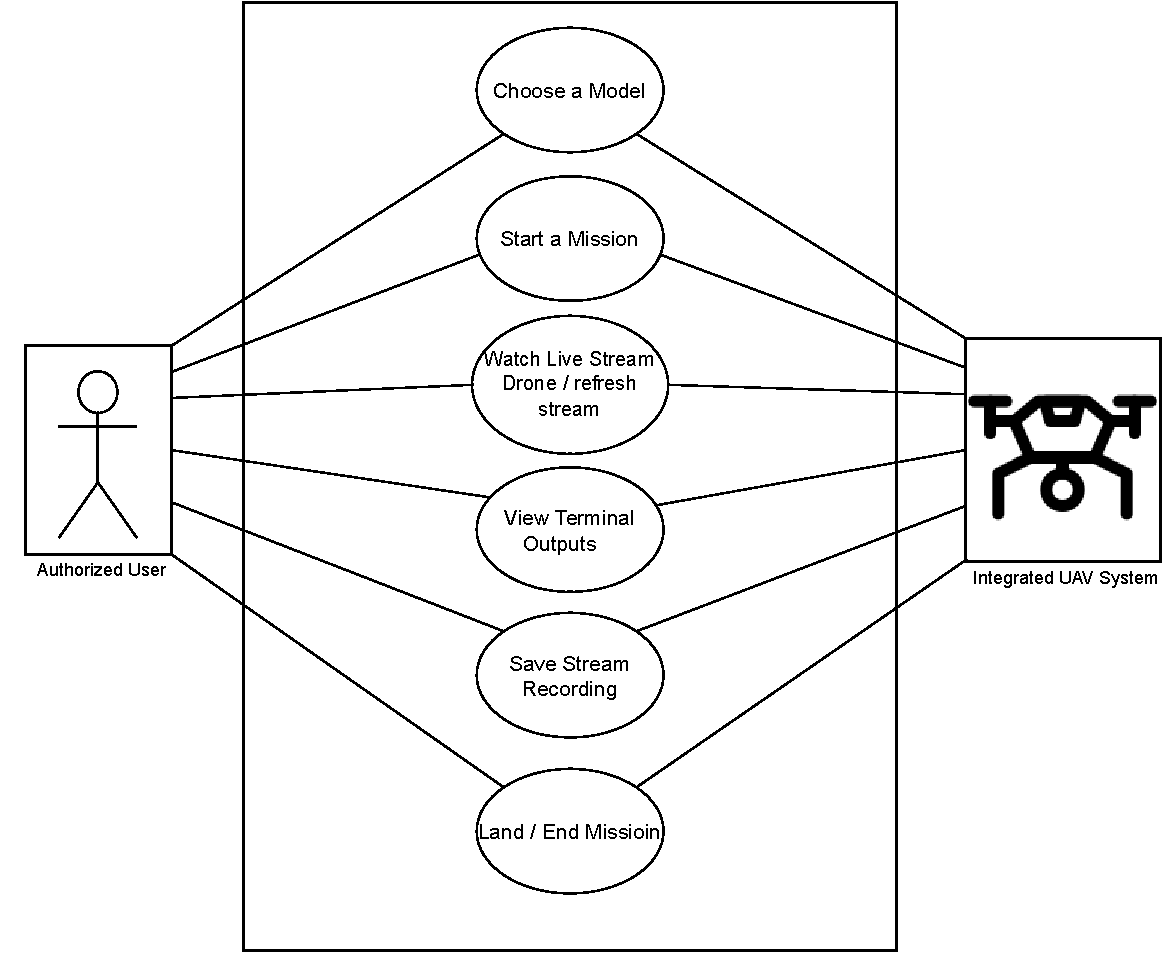
\includegraphics[width=0.9\textwidth]{gui-use-cases} 
	\caption{This use case diagram depicts the different use cases that any authorized users can have using the website.}
	\label{fig:gui-use-cases} 
\end{figure}

Below are the list of use cases that a user can do using the AirEye website as seen in \cref{fig:gui-use-cases} : 
\begin{itemize}	
	\item The user is able to choose a certain model that is available, choosing this model will run a specific script in the drone. 
	\item The user can start the mission.
	\item The user can watch the live stream from the drone camera and refresh the stream in case of any error.
	\item The user can see the outputs of the terminal to keep track of different variables.
	\item The user can save the stream recording. 
	\item The user can end the mission.
\end{itemize}

\begin{figure}[tbp]
	\centering
	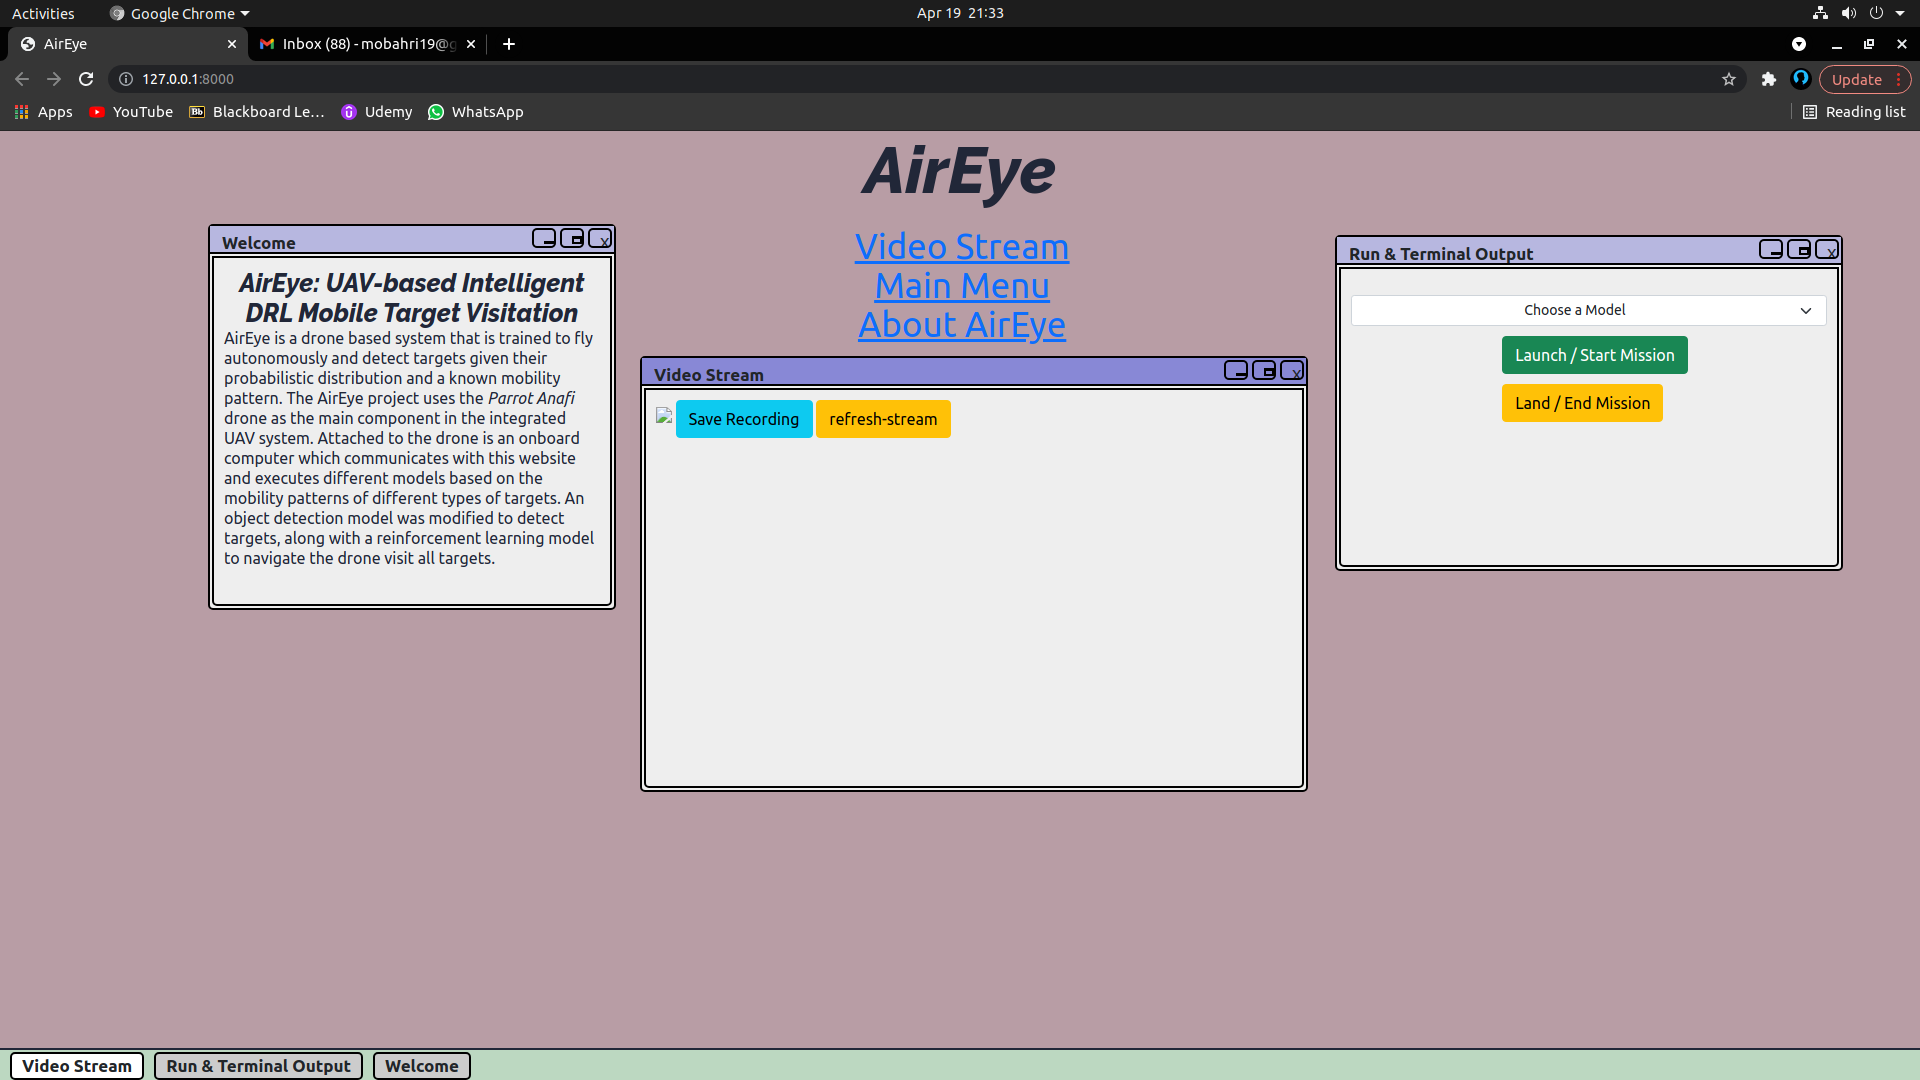
\includegraphics[width=0.99\textwidth]{gui-main-page}
	\caption{The main page of the AirEye website.}
	\label{fig:gui-main-page}
\end{figure}

Many software components were put together to produce what we have in \cref{fig:gui-main-page}, mainly: 
\begin{itemize}
	\item Olympe, the drone controller. 
	\item pyzbar, for \textsc{qr} code detection.
	\item OpenCV, huge computer vision library.
	\item \textsc{html}, \textsc{css}, and javascript for frontend web 
	development.
	\item Python Flask, backend framework.
	\item Gunicorn, \textsc{wsgi} \textsc{http} server
	\item Nginx, reverse proxy and web server. 
\end{itemize}

Many novel aspects were implemented in this website, different models could be 
made and each model is responsible for a certain type of targets, One model 
might be good for mobile targets and another could be better for fixed ones. 
Challenges were mainly faced in the backend as establishing the communication 
between the web server and the frontend was not easy to manage. Also, 
streaming live from the drone's camera to the user interface was 
difficult and new to us.



\end{document}
